\section{Nombre: Plataforma que desaparece.}\label{obs.PlatDes}
	\subsection{Descripción}
Porción de suelo que aparece y desaparece de manera periódica. Esta plataforma mantiene todas sus propiedades físicas mientras es visible, por lo que el jugador puede pararse sobre ella, pero, una vez desaparece el jugador caerá al vació si estaba parado sobre ésta. El jugador deberá saltar sobre ella y saltar fuera de ella para alcanzar terreno firme antes que desaparezca.  
	\subsection{Esquema}
Ver figura \ref{fig:plades}.
	\begin{figure}
  \centering
  \subfigure[La plataforma se muestra en el área de juego.]{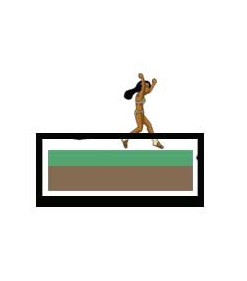
\includegraphics[width=0.3 \textwidth]{Imagenes/platDes}}
   \subfigure[Después de un tiempo la plataforma desaparece.]{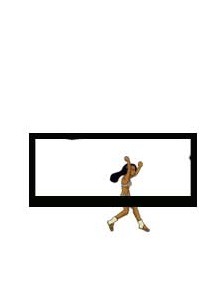
\includegraphics[width=0.2 \textwidth]{Imagenes/platDes02}}
    \subfigure[La plataforma vuelve a aparecer.]{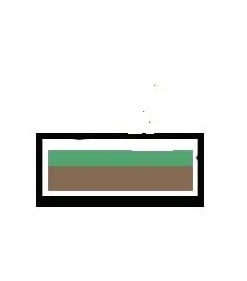
\includegraphics[width=0.3 \textwidth]{Imagenes/platDes03}}
  \caption{Plataforma que cae.}
  \label{fig:plades}
\end{figure}